% !TEX TS-program = xelatex
% !TEX encoding = UTF-8


\documentclass{beamer}

\graphicspath{{figures/}}


%\usepackage[adobefonts]{ctex}
%\setCJKmainfont{SimSun}
%\setsansfont{Times New Roman}



%%%%字体配置%%%%

\usepackage{xeCJK}
\setmainfont{Times New Roman}    % 缺省字体
\setsansfont{Times New Roman}

\setCJKmainfont[BoldFont={Adobe Heiti Std},ItalicFont={Adobe Kaiti Std}]{Adobe Fangsong Std}
\setCJKsansfont{Adobe Heiti Std}
\setCJKmonofont{Adobe Kaiti Std}
\setCJKfamilyfont{song}{Adobe Song Std}
\setCJKfamilyfont{hei}{Adobe Heiti Std}
\setCJKfamilyfont{kai}{Adobe Kaiti Std}
\setCJKfamilyfont{fs}{Adobe Fangsong Std}
%\setCJKfamilyfont{li}{LiSu}
%\setCJKfamilyfont{you}{YouYuan}
%\setCJKfamilyfont{yahei}{Microsoft YaHei}
%\setCJKfamilyfont{xingkai}{STXingkai}
%\setCJKfamilyfont{xinwei}{STXinwei}
%\setCJKfamilyfont{fzyao}{FZYaoTi}
%\setCJKfamilyfont{fzshu}{FZShuTi}
%
%-------------------------------------------------------------------
\newCJKfontfamily\song{Adobe Song Std}
\newCJKfontfamily\hei{Adobe Heiti Std}
\newCJKfontfamily\kai{Adobe Kaiti Std}
\newCJKfontfamily\fs{Adobe Fangsong Std}
%\newCJKfontfamily\li{LiSu}
%\newCJKfontfamily\you{YouYuan}
%\newCJKfontfamily\yahei{Microsoft YaHei}
%\newCJKfontfamily\xingkai{STXingkai}
%\newCJKfontfamily\xinwei{STXinwei}
%\newCJKfontfamily\fzyao{FZYaoTi}
%\newCJKfontfamily\fzshu{FZShuTi}

\XeTeXlinebreaklocale "zh"
\XeTeXlinebreakskip = 0pt plus 1pt minus 0.1pt

%%%%以上为字体配置

\usepackage{graphicx}
\usepackage{tabularx}
%\usepackage{fix-cm}
%\usepackage{color}
%
%\definecolor{title}{RGB}{128,128,128}




%%%%%%%

\usepackage{amssymb,latexsym,amssymb,amsmath,amsbsy,amsopn,amstext,upgreek}
\usepackage{color,multicol}
\usepackage{graphicx,wrapfig,fancybox,watermark,graphics}
%\usepackage{picins}
\usepackage{pgf}
%\usepackage{movie15}
%\usepackage{pdfpages}

%\usepackage{listings,bera}
%\definecolor{keywords}{RGB}{255,0,90}
%\definecolor{comments}{RGB}{60,179,113}
%\lstset{language=C,
%    keywordstyle=\color{keywords},
%    commentstyle=\color{comments}\emph
%}
%\usepackage{algorithm}
%\usepackage{algorithmic}
%\renewcommand{\algorithmicrequire}{\textbf{Input:}}
%\renewcommand{\algorithmicensure}{\textbf{Output:}}

% reference entry
\usepackage{bibentry}
\usepackage[numbers]{natbib}

\usepackage[
    compress,
    %minimal,
    nonav,
    red,
    %gold,
    %numbers,
    %nologo,
    NBU,
]
{beamerthemeNBU}
%\usefonttheme{structuresmallcapsserif}

%%%%%%%%%%%


%\mode<presentation>
%{
%  \usetheme{hackd}
%  % or ...
%
%  \setbeamercovered{transparent}
%  % or whatever (possibly just delete it)
%}




%第一种格式\\
\renewcommand{\today}{\number\year 年 \number\month 月 \number\day 日}
%\today\\
%第二种格式\\
%\renewcommand{\today}{\CJKnumber\year 年 \CJKnumber\month 月 \CJKnumber\day 日}
%\today

\title{宁波大学Xe\LaTeX 的Beamer模板}
\subtitle{2013年修改香港理工模板所得}

\author{杜碧升}

%\institute{宁波大学\quad 商学院\\管理科学与工程系}
\institute{商学院\ 管理科学与工程系}

\date[2013年教师教学技能培训]{{\small \today}}

\usepackage{hyperref}
\hypersetup{
  bookmarksnumbered={true},% 书签附上章节编号
    colorlinks,
    citecolor=blue,
    filecolor=black,
    linkcolor=black,
    urlcolor=black,
  pdfauthor = {\author},
  pdfkeywords = {理论,研究},
  pdftitle = {\title},
  pdfsubject = {笔记},
  pdfpagemode = UseNone
 %   pdfpagemode=FullScreen, % show in full screen?
}

\setcounter{tocdepth}{1}  % 设置目录的深度到 subsection

\AtBeginSection[] 
{ 
    \begin{frame} 
        \frametitle{概要} 
        \tableofcontents[currentsection,hideothersubsections] 
    \end{frame} 
} 

%\AtBeginSubsection[]
%{
%  \begin{frame}<beamer>{概要}
%%    \tableofcontents[currentsection,currentsubsection]
%    \tableofcontents[currentsection]
%  \end{frame}
%}

%%%%%%%%%%%%%%%%
%\makeatletter
%def\tableofcontents{%
%  \begin{small}
%  \leftline {{\bfseries \contentsname\/}}
%  \setcounter{secnumdepth}{4}%
%  \setcounter{tocdepth}{3}%
%  {\@starttoc{toc}}%
%\end{small}
%}
%\makeatother
%%%%%%%%%%%%%%%%


%%%%%%%%%%为了删掉顶边导航条
%\setbeamertemplate{headline}
%{
%  \leavevmode%
%  \hbox{%
%%  \begin{beamercolorbox}[wd=.5\paperwidth,ht=2.25ex,dp=1ex,right,rightskip=1em]{section in head/foot}%
%%    \usebeamerfont{subsection in head/foot}\hspace*{2ex}%\insertshorttitle
%%  \end{beamercolorbox}%
%%  \begin{beamercolorbox}[wd=.5\paperwidth,ht=2.25ex,dp=1ex,left,leftskip=1em]{subsection in head/foot}%
%%    \usebeamerfont{section in head/foot}%\insertsectionhead
%%    \hspace*{2ex}
%%  \end{beamercolorbox}
%  }%
%  \vskip0pt%
%}
%%%%%%%%%%为了删掉顶边导航条


\begin{document}
%\CTEXnoindent

\begin{frame}
  \titlepage
\end{frame}

\begin{frame}
%  \footnotesize
  \frametitle{概要}
  \tableofcontents
\end{frame}


\section{课程特性及教学对象}

\begin{frame}
\frametitle{课程特性}

\begin{alertblock}{课程特性}
本课程是商学院运作管理的一门专业课。
\end{alertblock}


\end{frame}


\begin{frame}
\frametitle{教学对象}


\begin{block}{教学对象}
科技学院法商分院信息管理专业两个班约50人。
\end{block}
\pause
\begin{block}{对象特征}
基础较薄弱,且对运作管理的重要性认识不深。
\end{block} 

\end{frame}


\section{教材选择及教学策略}

\begin{frame}
\frametitle{教材选择}

\begin{block}{教材}
《供应链管理》,黎继子,机械工业出版社,2011年2月。
\end{block}

%\pause
\begin{block}{参考书}
  \begin{thebibliography}{10}
    
  \beamertemplatebookbibitems
  % Start with overview books.

  \bibitem{Levi2010}
    大卫·辛奇-利维, 等。
    \newblock {\em 供应链设计与管理:概念、战略与案例研究(第3版) }.
    \newblock 中国人民大学出版社,2010年2月。

  \bibitem{Bozarth2008}
    Cecil Bozarth, Robert B. Handfield.
    \newblock {\em Introduction to Operations and Supply Chain Management. 2nd Ed, }.
    \newblock PEARSON, 2008

  \end{thebibliography}

\end{block}

\end{frame}


\begin{frame}
\frametitle{教学策略}

\begin{itemize}
\item 教学手段:采用课件演示、案例分析、思维游戏的方式。
%\pause
\item 教学方法:数学知识、理论模型对于三本学生来说,往往困难很大,教学时力求从学生身边的实例讲起,鼓励学生参与教学活动,通过案例分析的方式,分讨论组,布置学生课后资料整理,同时课上留出部分时间讨论,讨论的结果用演示文档做好并演讲,作为学生平时成绩的一部分。
\end{itemize}
\end{frame}



\section{重点难点及教学目标}


\begin{frame}
\frametitle{教学目标}

\begin{itemize}
\item 首先,理解概念。
%\pause
\item 其次,掌握架构。
%\pause
\item 第三,适当做题。
%\pause
\item 第四,理清脉络。
\end{itemize}

\end{frame}




\section{考核方式}

\begin{frame}
\frametitle{考核方式}

\begin{itemize}
\item 平时考核:考勤、课堂提问、小组讨论、演讲表现等。
%\pause
\item 案例报告:综合各成员成果分小组提交案例分析报告。
%\pause
\item 期末考试:在学期末统一闭卷考试。
\end{itemize}

%\pause
\begin{block}{最终成绩}
总成绩=25\%平时成绩+75\%($\frac{1}{3}$报告成绩+$\frac{2}{3}$期末成绩)
\end{block}

\end{frame}

\begin{frame}
\frametitle{为什么学习供应链管理?}

\begin{enumerate}
\item 无处不在(Pervasiveness)
%\pause
\item 互相依赖(Interdependence)
%\pause
\item 利润生存(Profitability and survival)
\end{enumerate}

\end{frame}


\begin{frame}
\frametitle{原因1:无处不在}

每一个组织都要为有价值的顾客\textbf{制造产品}或者\textbf{提供服务}。

\begin{block}{运作管理}

通过对一个公司内的人、技术和系统的合作,将投入通过\textbf{规划}、\textbf{调度}和\textbf{控制}等活动,来达到为组织提供\textbf{产品}和\textbf{服务}的过程。

\end{block}

\end{frame}


\begin{frame}
    \frametitle{背景、意义与研究现状}
    \begin{columns}
        \pause

        \column{.5\textwidth}
        \begin{itemize}
            \item 基于树状结构的检索
            \begin{itemize}
                \item 基于路径索引
            \end{itemize}
        \end{itemize}

        \pause

        \column{.5\textwidth}    
        \begin{itemize}
            \item<2-> 搜索引擎
            \item<4-> MathML
              \begin{itemize}
                \item<4-> Content MathML
                \item<4-> Presentation MathML
              \end{itemize}
            \item<3-> MongoDB
        \end{itemize}

    \end{columns}
\end{frame}


\begin{frame}

插入图片如下图
\begin{figure}[htbp] 
\centering
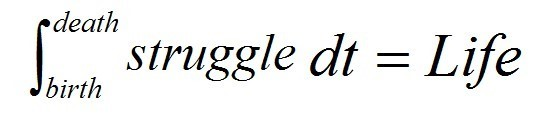
\includegraphics[width=0.95\textwidth]{test} 
%\caption{something}
%\label{fig:1} 
\end{figure} 


插入公式并且放大到文本宽度如下:
\vspace{0.5cm}

%\resizebox{\textwidth}{!}{$a+b=c$}

\resizebox{\textwidth}{!}{
%\begin{equation*}
  $\int_{\tt birth}^{\tt death} {\tt struggle}\ {\tt d}t = {\tt Life}$
%\end{equation*}
}

\end{frame}

\section*{}

\begin{frame}
    \vspace{4cm}

    \bf \Huge{
        \begin{tabularx}{\textwidth}{c}
            \makebox[\textwidth]{\hfill \color{NBUred}{敬请批评指正!} \hfill}
        \end{tabularx}
    }

    \vspace{4cm}

    \bf \Huge{
        \begin{tabularx}{\textwidth}{c}
            \makebox[\textwidth]{\hfill \color{NBUred}{\hei 敬请批评指正!} \hfill}
        \end{tabularx}
    }
    
\end{frame}


\plainframe{
%\begin{frame}
%\frametitle{Q \& A}
  \begin{center}
    \Huge \color{NBUred}{谢谢!}   %\\
%    \Huge \color{cyan}{Q \& A}
  \end{center}
%\end{frame}
}



\end{document}